% Fig 2.2 — Query Enhancement taxonomy
% Tree showing where Query2Doc, HyDE, GAR, GRF, CSQE sit; dashed box marks "this thesis".

\documentclass[border=4pt]{standalone}
\usepackage{tikz}
\usetikzlibrary{positioning, arrows.meta, shapes.geometric, fit, backgrounds}

\begin{document}
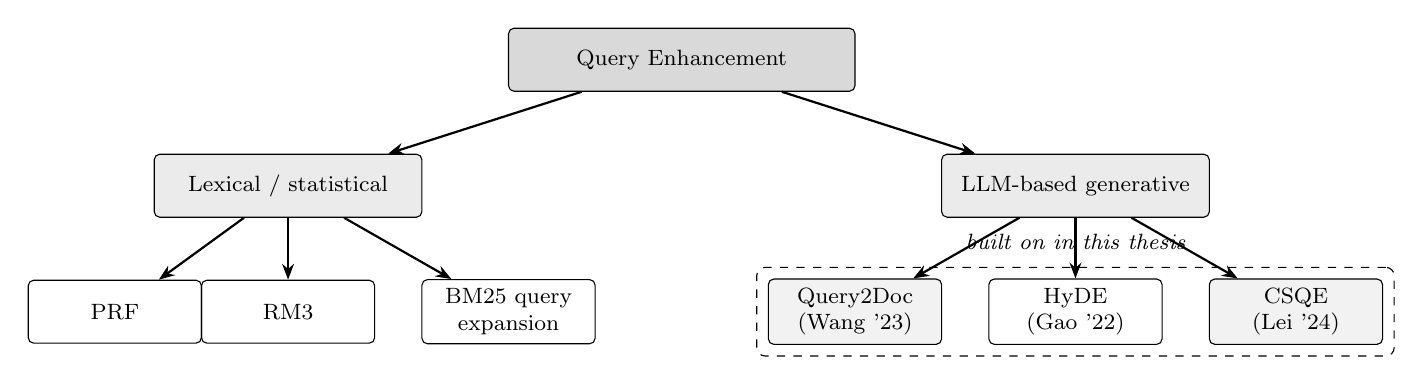
\begin{tikzpicture}[
    >=Stealth,
    box/.style={rectangle, draw, rounded corners=2pt,
                minimum width=24mm, minimum height=8mm,
                align=center, font=\footnotesize},
    root/.style={box, fill=black!15, minimum width=44mm},
    branch/.style={box, fill=black!8, minimum width=34mm},
    leaf/.style={box, minimum width=22mm},
    thesis/.style={leaf, fill=black!5},
    arrow/.style={-{Stealth[length=2mm]}, thick}
]
  \node[root] (root) at (0, 0) {Query Enhancement};

  % Two branches
  \node[branch] (lex) at (-50mm, -16mm) {Lexical / statistical};
  \node[branch] (gen) at (50mm, -16mm) {LLM-based generative};

  % Lexical leaves
  \node[leaf] (prf) at (-72mm, -32mm) {PRF};
  \node[leaf] (rm3) at (-50mm, -32mm) {RM3};
  \node[leaf] (bm25exp) at (-22mm, -32mm) {BM25 query\\expansion};

  % Generative leaves
  \node[thesis] (q2d) at (22mm, -32mm) {Query2Doc\\(Wang '23)};
  \node[leaf] (hyde) at (50mm, -32mm) {HyDE\\(Gao '22)};
  \node[thesis] (csqe) at (78mm, -32mm) {CSQE\\(Lei '24)};

  % Edges from root
  \draw[arrow] (root) -- (lex);
  \draw[arrow] (root) -- (gen);

  % Edges from lex
  \draw[arrow] (lex) -- (prf);
  \draw[arrow] (lex) -- (rm3);
  \draw[arrow] (lex) -- (bm25exp);

  % Edges from gen
  \draw[arrow] (gen) -- (q2d);
  \draw[arrow] (gen) -- (hyde);
  \draw[arrow] (gen) -- (csqe);

  % "This thesis" box around Q2D + CSQE
  \begin{scope}[on background layer]
    \node[draw, dashed, rounded corners=3pt, fit=(q2d) (csqe), inner sep=4pt] (thesisbox) {};
  \end{scope}
  \node[font=\footnotesize\itshape, above=1mm of thesisbox] {built on in this thesis};
\end{tikzpicture}
\end{document}
